%% entwurf.tex
%% $Id: entwurf.tex 28 2007-01-18 16:31:32Z bless $
%%
%% ==============================
\chapter{Design}
\label{ch:Design}

\section{Prototype}

For the recording of the temperature at different positions of the ear, an own prototype was developed within the scope of this master thesis.
This is based on OpenEarable, a platform developed by TECO for ear-based temperature measurements.
The prototype consists of 2 parts, an earpiece, which resembles an in-ear headphone, and a component behind the ear, which reminds of a hearing aid.
The OpenEarable is placed in the component behind the ear, as well as the PCB, to which three temperature sensors are connected to measure the temperature behind the ear.
The second component in the ear is connected to the OpenEarable via I2C.
The OpenEarable serves as a base to read and store the data of the sensors connected via I2C.
The relationship and the interaction of the components are visually highlighted in Figure \ref{fig:design:prototype_connection}.
For each of the parts, the housing was printed with a 3D printer after being created with TinkerCAD.
% TODO: add pictures of the 3D printed results if available

\begin{figure}[t]
    \centering
    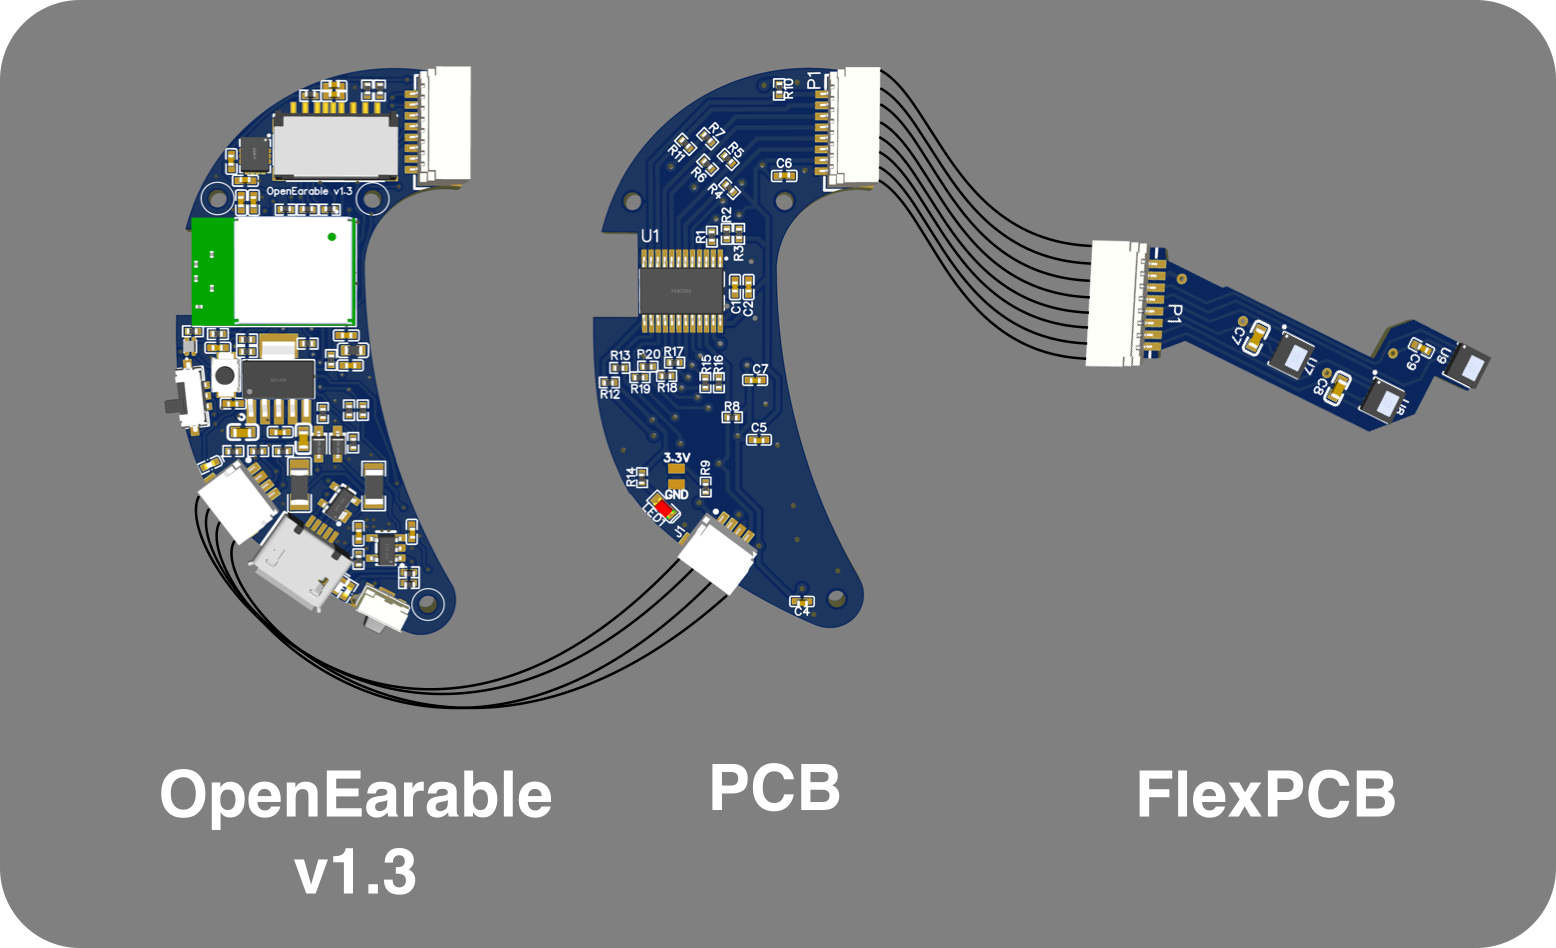
\includegraphics[width=\textwidth]{thesis-doc/images/prototype/PrototypeConnection.png}
    \caption{Visual representation of the prototype and the interaction of all components. The PCB is connected to the OpenEarable v1.3 with a 4-pin connector. In the OpenEarable is an Arduino Nano33 BLE, with which it is possible to control the multiplexer (TCA9548A) via I2C. Through this, every sensor value on the PCB and also on the FlexPCB can be read out, since the FlexPCB is also connected to the multiplexer via the 8-pin connector.}
    \label{fig:design:prototype_connection}
\end{figure}

\subsubsection{Temperature measurements behind the ear}

The temperature behind the ear is measured at 3 positions, as can be seen in Figure \ref{fig:design:pcb_description}.
To position the temperature sensors at the locations, a PCB was developed that has the sensors installed at the appropriate locations. 
The PCB is located at the very bottom directly on the case so that the sensors can measure the temperature through the locations exposed on the case.
The sensor used requires an angle of $ 50 ^ \circ$ around itself for the temperature to be reliably measured. 
This was taken into account.
Above the PCB, the battery is placed in the enclosure so that no long cables are needed for the power supply to record the data in the study conducted.
The OpenEarable is placed above this.
The dimensions of the PCB are exactly the same as the OpenEarable to keep the case as small and compact as possible.
The PCB has a TCA9548A multiplexer, to which the MLX90632 sensors are connected.
These can now be addressed and read out individually.
The PCB also has 3 more sensors connected via the multiplexer, but they lead away from the PCB.
Via an 8-pin connector, a cable leads a connection to the second component, the earpiece.
Here 3 more temperature sensors are connected, which can also be addressed with the multiplexer.

\begin{figure}[t]
    \centering
    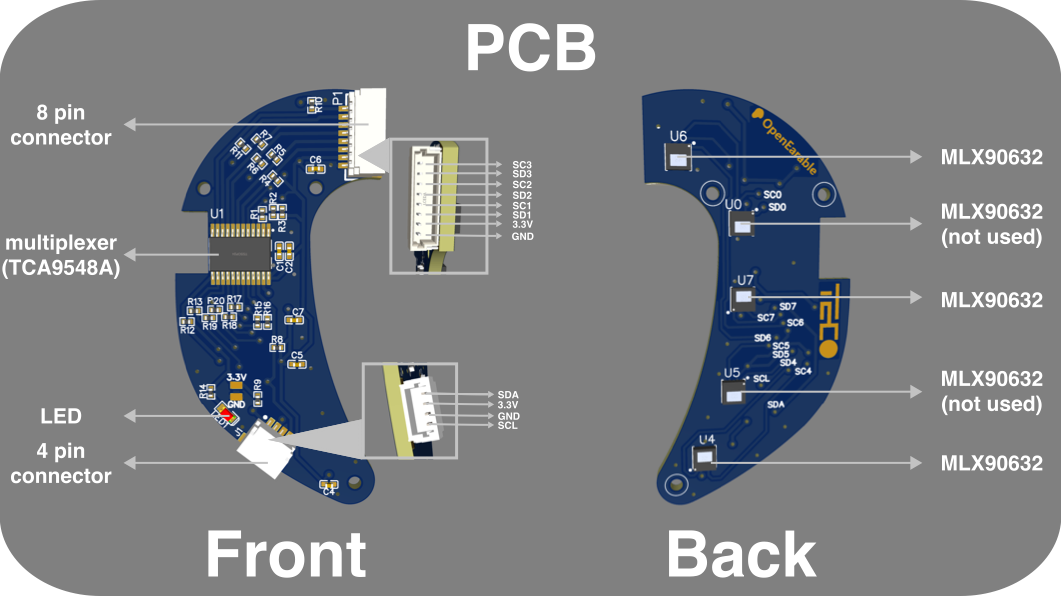
\includegraphics[width=\textwidth]{thesis-doc/images/prototype/PCB_Description.png}
    \caption{Representation of the front and back of the PCB. The multiplexer can be seen on the front, which is controlled by the OpenEarable via the 4-pin connector. The three other MLX90632 are then connected by the FlexPCB via the 8-pin connector. In addition, an LED is connected to the front, which lights up green if no short circuit is generated. The temperature sensors can be seen on the back, but only three of the five connections visible in the design are used.}
    \label{fig:design:pcb_description}
\end{figure}

\subsubsection{Temperature measurements in the ear}

The 2nd component now enables the temperature measurement in the ear.
With an 8-pin connector, the component can be connected to the board, which was just described in the \ref{TODO REF} section.
The part is based on the design of an Airpod, but heavily modified.
The design is freely available on TinkerCAD and was used to have a suitable shape available as a basis for the part.
The design was completely hollowed out from the inside to allow wires to be placed through the case.
In addition, an adapter was attached to the side where the Airpod fits into the ear. 
An adapter was attached here, which can then be used to attach an earplug.
This ensures that the earplug protrudes further into the ear than usual compared to conventional in-ear headphones.
This serves to make a temperature measurement in the direction of the eardrum. 
This is achieved by attaching a temperature sensor to the tip of the earplug to record the ground truth of the measurement. 
The temperature sensor is located next to 2 other temperature sensors on a FlexPCB, which was also designed.
This is connected to the PCB via the 8-pin port, which is placed behind the ear.
The 3 temperature sensors on the FlexPCB can be switched via the multiplexer, which is connected to the PCB.
In addition to the temperature sensor to measure the temperature of the tympanic membrane, a temperature sensor was also attached to measure the temperature of the ear canal and the pinna. 
These are attached to the FlexPCB and mounted on the component to measure the temperature at the appropriate positions.

TODO: create images for visual clearance

\subsection{sensors}

Based on research and experience at the TECO Institute, the MLX90632 sensor was selected for its suitability for our project.

The MLX90632 sensor is an infrared temperature sensor known for its high accuracy in temperature measurements. This enables reliable applications where precise temperature tracking is needed.
Furthermore, non-contact temperature measurement is a huge advantage. The MLX90632 can measure temperature without physical contact with the object or body part, providing a non-invasive and convenient ear temperature monitoring option.
In order to place the temperature sensors in the necessary locations to measure temperature, the sensors must be appropriately small. Since the MLX90632 has a small form factor, this is optimal for the application needed.
Additionally, the MLX90632 is readily available on the market and has existing Arduino libraries. This availability and compatibility with Arduino simplify the integration process and save valuable development time.
In addition, the sensor is designed for low power consumption, making it suitable for battery-powered devices. Given the small battery size in the developed prototype, low power consumption is critical for extended operation during the study.
The MLX90632 offers fast response times and allows for real-time temperature monitoring and fast updates. Some difficulties arose when writing the EEPROM, so the default value was left at 2Hz.
The intention of adjusting the measuring rate was the implementation details of the library, which was finally solved by adjusting the library. This process is described in more detail in the chapter \ref{TODO: ann ref}.
The high sensitivity to temperature changes allows the MLX90632 to accurately detect even minor variations. This sensitivity is advantageous for precise temperature tracking.
In addition, the sensor has applications in both the consumer and industrial markets due to its accuracy and reliability. This versatility makes it an excellent choice for our master's thesis project, which involves working with an Arduino Nano 33 BLE.
Overall, the infrared temperature sensing capabilities, accuracy, easy availability, non-invasive measurement, compact size, and compatibility with Arduino make the MLX90632 an ideal choice for the developing ear temperature monitoring system.

\subsection{Platform: OpenEarable}

In chapter \ref{Background:SensingWithEarables:OpenEarable} the OpenEarable platform is described in detail. 
Here, the interaction with the other components is focused.

% TODO: Auch explizit die Pin belegung mit beschreiben

% TODO: Grafik mit mit PCB, wie die alle connected sind über die PIN anschlüsse

PCB Design, FlexPCB, how everything interacts, especially with OpenEarable.
% TODO: PCB Schematic in den Anhang vermutlich packen, sehr wichtig!!!

\section{study}